\section{Installation du programme {\nomLogiciel}}

\subsection{Configuration de la Raspberry Pi}
\subsubsection{Configuration du bus CAN}
Si vous récupérez une Raspberry Pi neuve, il y aura un certain nombre de configurations à faire avant de pouvoir faire fonctionner le programme {\nomLogiciel}. Vous pouvez également vous servir des informations suivantes pour vérifier que la Raspberry Pi que vous avez est correctement configurée.\\

Commencez par placer le RS485 CAN Hat sur la Raspberry Pi. \\

\textbf{Attention, si vous souhaitez utiliser le Banc de Test, il vous faut un RS485 CAN Hat sans résistance de terminaison.}\\

Le protocole CAN utilise le bus SPI pour communiquer, il faut donc configurer votre Raspberry Pi pour qu'elle active ce bus.
Pour cela, éditez le fichier config.txt (en root) :
\vspace{-1.8\baselineskip} 
\begin{lstlisting}
    sudo nano /boot/config.txt
\end{lstlisting} 
Parcourez le fichier, si vous ne les trouvez pas, tapez les lignes suivantes :
\vspace{-1.8\baselineskip} 
\begin{lstlisting}
    dtparam=spi=on
    dtoverlay=mcp2515-can0,oscillator=12000000,interrupt=25,spimaxfrequency=2000000
\end{lstlisting}
Redémarrez la Raspberry Pi :
\vspace{-1.8\baselineskip} 
\begin{lstlisting}
    sudo reboot
\end{lstlisting}

Maintenant que le bus SPI est fonctionnel, il reste à configurer le bus CAN.
Commencez par installer le package qui permettra de configurer le bus CAN :
\vspace{-1.8\baselineskip} 
\begin{lstlisting}
    sudo apt install can-utils
\end{lstlisting}
Afin de faciliter l'utilisation de la Raspberry Pi, voici un tutoriel pour que le bus CAN se configure correctement à chaque démarrage de la Raspberry Pi :
\begin{enumerate}
    \item Créez un fichier can0.service et éditez le : 
\vspace{-1.8\baselineskip} 
\begin{lstlisting}
    touch /etc/systemd/system/can0.service
    sudo nano /etc/systemd/system/can0.service
\end{lstlisting}
    \item Ecrivez les lignes suivantes et sauvegardez : 
\vspace{-1.8\baselineskip} 
\begin{lstlisting}
    [Unit]
    Description=CAN0 interface initialization

    [Service]
    ExecStart=/bin/bash -c "/sbin/ifconfig can0 down && /sbin/ip link set can0 type can bitrate 125000 && /sbin/ifconfig can0 up"

    [Install]
    WantedBy=multi-user.target
\end{lstlisting}
    \item Tapez la ligne suivante pour activer le service :
\vspace{-1.8\baselineskip} 
\begin{lstlisting}
    sudo systemctl enable can0.service
\end{lstlisting}
    \item Redémarrez la Raspberry Pi. \newline
\end{enumerate}

Après le démarrage de la Raspberry Pi, vous pouvez vérifier que le service s'est correctement lancé en tapant :
\vspace{-1.8\baselineskip} 
\begin{lstlisting}
    systemctl status can0.service
\end{lstlisting}
Vous devriez voir apparaître ceci :
\vspace{-1.8\baselineskip} 
\begin{lstlisting}
    can0.service - CAN0 interface initialization
     Loaded: loaded (/etc/systemd/system/can0.service; enabled; vendor preset: enabled)
     Active: inactive (dead) since Mon 2023-06-05 19:53:59 CEST; 22min ago
    Process: 350 ExecStart=/bin/bash -c /sbin/ifconfig can0 down && /sbin/ip link set can0 type can bitrate 125000 && /sbin/ifconfig can0 up (code=exited, status=0/SUCCESS)
    Main PID: 350 (code=exited, status=0/SUCCESS)
            CPU: 54ms

    juin 05 19:53:59 raspberrypi systemd[1]: Started CAN0 interface initialization.
    juin 05 19:53:59 raspberrypi systemd[1]: can0.service: Succeeded.
\end{lstlisting}

Vous pouvez connaître l'état du bus CAN grâce à cette commande :
\vspace{-1.8\baselineskip} 
\begin{lstlisting}
    sudo ip -details link show can0
\end{lstlisting}

Le bus peut être dans divers états : \\
\begin{minipage}
    \textwidth
    \centering
    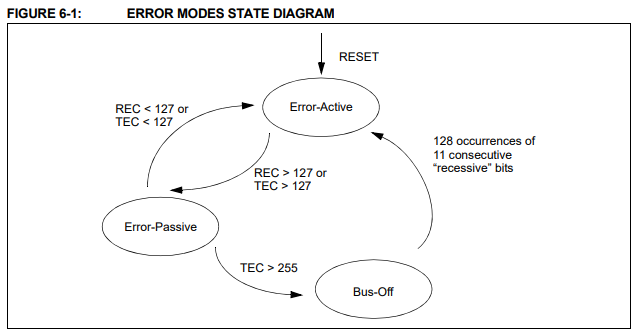
\includegraphics{../figures/Etat_CAN.png}
    \captionof{figure}{Diagramme d'état des modes d'erreurs (extrait de la datasheet du MCP2515)}
\end{minipage}

\medspace

Lorsque le bus est éteint, il est dans l'état STOPPED :
\vspace{-1.8\baselineskip} 
\begin{lstlisting}
    3: can0: <NOARP,UP,LOWER_UP,ECHO> mtu 16 qdisc pfifo_fast state UP mode DEFAULT group default qlen 10
    link/can  promiscuity 0 minmtu 0 maxmtu 0 
    can state STOPPED (berr-counter tx 0 rx 0) restart-ms 0 
	  bitrate 125000 sample-point 0.875 
	  tq 500 prop-seg 6 phase-seg1 7 phase-seg2 2 sjw 1
	  pcan_usb: tseg1 1..16 tseg2 1..8 sjw 1..4 brp 1..64 brp-inc 1
	  clock 8000000 numtxqueues 1 numrxqueues 1 gso_max_size 65536 gso_max_segs 65535 parentbus usb parentdev 2-2.1:1.0  
\end{lstlisting}


Lorsque le bus est fonctionnel, il est dans l'état ERROR-ACTIVE :
\vspace{-1.8\baselineskip} 
\begin{lstlisting}
    3: can0: <NOARP,UP,LOWER_UP,ECHO> mtu 16 qdisc pfifo_fast state UP mode DEFAULT group default qlen 10
    link/can  promiscuity 0 minmtu 0 maxmtu 0 
    can state ERROR-ACTIVE (berr-counter tx 0 rx 0) restart-ms 0 
	  bitrate 125000 sample-point 0.875 
	  tq 500 prop-seg 6 phase-seg1 7 phase-seg2 2 sjw 1
	  pcan_usb: tseg1 1..16 tseg2 1..8 sjw 1..4 brp 1..64 brp-inc 1
	  clock 8000000 numtxqueues 1 numrxqueues 1 gso_max_size 65536 gso_max_segs 65535 parentbus usb parentdev 2-2.1:1.0  
\end{lstlisting}

Lorsque le bus est en erreur, il est dans l'état ERROR-PASSIVE :
\vspace{-1.8\baselineskip} 
\begin{lstlisting}
    3: can0: <NOARP,UP,LOWER_UP,ECHO> mtu 16 qdisc pfifo_fast state UP mode DEFAULT group default qlen 10
    link/can  promiscuity 0 minmtu 0 maxmtu 0 
    can state ERROR-PASSIVE (berr-counter tx 0 rx 0) restart-ms 0 
	  bitrate 125000 sample-point 0.875 
	  tq 500 prop-seg 6 phase-seg1 7 phase-seg2 2 sjw 1
	  pcan_usb: tseg1 1..16 tseg2 1..8 sjw 1..4 brp 1..64 brp-inc 1
	  clock 8000000 numtxqueues 1 numrxqueues 1 gso_max_size 65536 gso_max_segs 65535 parentbus usb parentdev 2-2.1:1.0  
\end{lstlisting}
Dans cet état, il faut redémarrer le bus pour qu'il recommence à fonctionner. Pour cela, vous pouvez soit redémarrer la Raspberry Pi (dans le cas où le service est "enable" et se lance tout seul au boot de la Raspberry Pi), soit taper la commande : 
\vspace{-1.8\baselineskip} 
\begin{lstlisting}
    sudo systemctl restart can0.service
\end{lstlisting}

\subsubsection{Installation du Hotspot}
Afin de permettre au Smartphone de se connecter à la Raspberry Pi, il lui faut générer un Hotspot. 

Pour cela, vous pouvez suivre le tutoriel de ce site : \href{https://bentek.fr/creer-hotspot-wifi-sur-raspberry-pi/}{Créer un hotspot sur Raspberry Pi}.
\begin{enumerate}
    \item Installez RaspAP : \newline
    Création d'une sauvegarde du fichier de configuration WiFi :
\vspace{-1.8\baselineskip} 
\begin{lstlisting}
    sudo cp /etc/wpa_supplicant/wpa_supplicant.conf /etc/wpa_supplicant/wpa_supplicant.conf.sav
\end{lstlisting}
    Suppression du fichier de configuration WiFi pour retourner à une configuration vierge :
\vspace{-1.8\baselineskip} 
\begin{lstlisting}
    sudo cp /dev/null /etc/wpa_supplicant/wpa_supplicant.conf
\end{lstlisting}
    Téléchargement et installation de RaspAP :
\vspace{-1.8\baselineskip} 
\begin{lstlisting}
    wget -q https://git.io/voEUQ -O /tmp/raspap && bash /tmp/raspap
\end{lstlisting}
    \item Attendez la fin du téléchargement et redémarrez la Raspberry Pi.\newline
\end{enumerate}

Ce réseau est automatiquement déployé sur wlan0. Vous pouvez taper la commande suivante pour vérifier que le hotspot est en place : 
\vspace{-1.8\baselineskip} 
\begin{lstlisting}
    ip a
\end{lstlisting}
Vous devriez voir à minima :
\vspace{-1.8\baselineskip} 
\begin{lstlisting}
    wlan0: <BROADCAST,MULTICAST,UP,LOWER_UP> mtu 1500 qdisc pfifo_fast state UP group default qlen 1000
    link/ether b8:27:eb:7d:39:15 brd ff:ff:ff:ff:ff:ff
    inet 10.3.141.1/24 brd 10.3.141.255 scope global noprefixroute wlan0
       valid_lft forever preferred_lft forever
    inet6 fe80::bc4f:144b:a962:a45f/64 scope link 
       valid_lft forever preferred_lft forever
\end{lstlisting}

Vous pouvez connecter votre Smartphone ou votre PC au hotspot, le nom du réseau est "raspi-webgui". Le mot de passe est "ChangeMe".

L'interface d'adminitration de RaspAP est accessible en vous connectant au hotspot, tapez "10.3.141.1" dans un navigateur web. Par défaut, le nom d'utilisateur est "admin" et le mot de passe est "secret". Vous pouvez configurer le hotspot à votre convenance.

\subsection{Installation des outils pour compiler le programme {\nomLogiciel}}

\subsubsection{Installation du compilateur}

Afin de compiler le programme pour Raspberry Pi, il faut installer le compilateur ARM. Vous pouvez utiliser celui que vous souhaitez mais nous vous proposons ce tutoriel pour récupérer le compilateur utilisé lors du développement :
\begin{enumerate}
    \item Récupérer les outils de développement croisés : \newline
    Dans le dossier de votre choix, tapez la commande suivante :
\vspace{-1.8\baselineskip} 
\begin{lstlisting}
    git clone https://github.com/raspberrypi/tools.git
\end{lstlisting}
    \item Modifier le fichier "variable.mk" afin de renseigner le chemin absolu vers le compilateur (dossier où vous avez cloné le fichier précédemment) : modifez la variable "RASPBERRY\_TOOLS". \newline
\end{enumerate}

Si ce n'est pas déjà fait, pensez également à installer gcc sur votre machine, dans n'importe quel terminal, tapez : 
\vspace{-1.8\baselineskip} 
\begin{lstlisting}
    sudo apt install gcc
\end{lstlisting}

\subsubsection{Installation de CMocka}

Le programme {\nomLogiciel} est fourni avec des tests automatisés. Afin de compiler ces tests, vous avez besoin de la librairie CMocka. Les tests sont autant exécutables sur votre machine que sur cible. Si votre machine ne possède pas la même architecture que la Raspberry Pi, vous avez donc besoin de deux librairies différentes. Afin de faciliter l'utilisation de CMocka, nous vous proposons de compiler la librairie en statique. \newline

Le tutoriel est le même pour les deux architectures, la seule différence est que pour une compilation sur cible, vous devez compiler la librairie sur la cible, pour une compilation locale, vous devez compiler la librairie sur votre machine. \newline

Attention, afin de compiler la librairie, vous avez besoin de cmake et make, dans un terminal, tapez :
\vspace{-1.8\baselineskip} 
\begin{lstlisting}
    sudo apt install cmake
    sudo apt install make
\end{lstlisting}

\begin{enumerate}
    \item Téléchargez CMocka \href{https://cmocka.org/}{CMocka}, version 1.1.5.
    \item Consultez les fichier README et INSTALL pour plus d'informations sur l'installation de CMocka.
    \item Dans le fichier "DefineOptions.cmake" : 
\vspace{-1.8\baselineskip} 
\begin{lstlisting}
    option(WITH_STATIC_LIB "Build with a static library" ON)
\end{lstlisting}
    \item Créez un répertoire "build" dans le dossier de CMocka et allez dedans.
    \item Générez le Makefile avec cmake :
\vspace{-1.8\baselineskip} 
\begin{lstlisting}
    cmake -DCMAKE_INSTALL_PREFIX=<choisir un emplacement> ..
\end{lstlisting}
    \item Compilez et installez la librairie :
\vspace{-1.8\baselineskip} 
\begin{lstlisting}
    make
    make install
\end{lstlisting}
\end{enumerate}

Si vous avez compilez la librairie sur cible, vous pouvez récupérer les dossier "include" et "lib" dans le dossier d'installation que vous avez choisi et les installer sur votre machine. \newline
Vous pouvez utiliser la commande "scp" pour copier les dossiers de la cible vers votre machine :
Sur votre machine, tapez : 
\vspace{-1.8\baselineskip} 
\begin{lstlisting}
    scp -r <user>@<ip>:<chemin vers le dossier> <chemin vers le dossier de destination>
\end{lstlisting}

Après avoir récupéré les deux librairies, modifiez le fichier "variable.mk" afin de renseigner les chemins absolus vers les librairies : modifez la variable "CMOCKA" (Attention, elle est déclarée deux fois dans le fichier selon si la variable "TARGET" est égale à "raspberry" ou non).

\subsubsection{Compilation du programme {\nomLogiciel}}

Vous avez désormais tous les outils nécessaires pour compiler le programme {\nomLogiciel}. \newline

Comme expliqué précédemment, il est possible d'exécuter les tests automatisés sur cible et sur votre machine. \newline

Lorsque le programme est compilé sur cible, un script est appelé afin de transmettre l'exécutable à la Raspberry Pi. Pour que cela fonctionne, assurez-vous de pouvoir vous connecter à la Raspberry Pi en SSH. \newline

Vous pouvez modifier le fichier "transfert\_bin.sh" afin de renseigner le nom d'utilisateur et l'adresse IP de la Raspberry Pi. \newline
Dans le cas où votre Raspberry Pi aurait un port de connexion SSH différent de celui par défaut, pensez à modifier la commande "scp" du fichier afin de lui indiquer le port à utiliser : utilisez le paramètre "-P" suivi du numéro du port. \newline

Pour compiler : 
\begin{enumerate}
    \item Ouvrez un terminal dans le dossier "production". 
    \item Pour compiler sur cible, tapez :
\vspace{-1.8\baselineskip} 
\begin{lstlisting}
    make TARGET=raspberry
\end{lstlisting}
\newpage
    \item Pour compiler sur votre machine, tapez :
\vspace{-1.8\baselineskip} 
\begin{lstlisting}
    make 
\end{lstlisting}
\end{enumerate}

Une fois la compilation terminée, vous pouvez voir les exécutables "CANgateway.out" et "CANgateway\_test.out" dans le dossier "bin". \newline

Pour une compilation sur cible, les exécutables sont visibles dans le dossier /home/pi de la Raspberry Pi. \newline
